\Chapter{A tűz megjelenítése}

% TODO: Összeszedni az eddigi eredményeket a tűz megjelenítésével kapcsolatban!

\section{Megvalósítás a fontosabb játék motorokban}

A háromdimenziós játékok felemelkedése az 1990-es években kezdődött. Az első játékmotorok az id Software feljelszőinek köszönhetőek. Ahelyett, hogy minden játékot egyenként a semmiből építettek volna fel, más fejlesztők által készített modulokat használtak fel. Megtervezték a saját grafikájukat, karaktereiket, fegyvereiket és pályáikat, melyek lényegében a játék tartalmát nyújtották. Így már szét lehetett választani a játékspecifikus szabályokat és adatokat olyan alap koncepcióktól, mint például az ütközésvizsgálat. Ennek köszönhetően a fejlesztői csapatokat lehetett bővíteni, hiszen egyszerre több modulon is lehetett párhuzamosan, egymástól függetlenül dolgozni. Ez lehetővé tette továbbá, hogy a fejlesztők külön területekre specializálódjanak.
\cite{wikiGameEngine}

A korábbi, kétdimenziós játékokban természetesen csak sprite (kétdimenziós bitmap) alapú tüzekkel találkozhatunk. Az id tech 1 motor sem kivétel, habár hármodimenziósnak tűnnek a vele készült játékok (pl.: Doom I, Doom II), a benne lévő objektumok szintén sprite-ok, melyek mindig a néző felé fordulnak. Az ilyen játékmotorokat 2.5 dimenziós motoroknak is nevezhetjük. 


%Sprite tűz:
%1993 id tech 1/doom engine https://en.wikipedia.org/wiki/Doom_engine +  https://doomwiki.org/wiki/Doom_rendering_engine 
% Doom II: Hell on Earth (id tech 1 ez is)

\subsection{Quake engine 1996}
% MDL format: http://fabiensanglard.net/quakeSource/quakeSourceRendition.php
% torch animation http://media.moddb.com/images/members/1/240/239733/qv1.gif
A Quake motor 1996-ban készült el a Quake számítógépes játékot meghajtva. Az id tech 1 motorral ellentétben ez már igaz háromdimenziós motor, azaz háromdimenziós adatokat felhasználva állítja elő a kétdimenziós képet. A megjelenítés valós időben történik. A játékban egyaránt használtak fénytérképeket (lightmap) és 3D-s fényforrásokat is. Előbbi segítségével a statikus objektumok fényét lehetett az objektumokra égetni, ezzel rövidítve a kirajzolási időt, utóbbi pedig a dinamikus objektumok fényét adta. \cite{wikiQuake} A játékban a fáklyák tüzét vizsgáltam.

A tűz maga váltakozó modellek sorozatából állt, melyet MDL fájformátumban tároltak le.\\
 Ez a formátum lehetővé teszi a képkockáról képkockára való animáció tárolását. Egy .mdl fájl jellemzői: 
\begin{itemize} 
\item A modell geimetriai adatai (háromszögekben)
\item Textúra adatok
\item Képkockáról képkockára való animáció
\end{itemize} 
Egy MDL fájlban több textúra is lehet. Minden képkockához külön-külön hozzá lehet rendelni egyebek mellett, hogy mely csúcsok szerepelnek benne. A formátum lehetővé teszi egy befoglaló gömb megadását is, mely ütközésvizsgálatok esetén lehet fontos, ám ezt nem kötelező megadni benne.  \cite{MDLformat} 
 
Tehát a tűznek semmiféle külön fizikai modellezéséről sincs szó (legalábbis valós időben), előre meg van határozva a mozgása képkockákra lebontva. A fáklyák kaphattak pislákoló fényt, ám ez rendkívül lassította a kirajzolást, így többnyire csak olyan helyen lehetett alkalmazni ahol kevés felületet világított meg. Mint az a mellékelt ábrán is látszik, a tűz lángjain nem lehet átlátni, illetve füstképződés sincs. Kipróbálni nem tudtam, de az interneten fellelhető videók alapján arra a következtetésre jutottam, hogy a lánggal való ütközés nincs külön vizsgálva. Azt is sikerült megfigyelnem, hogy amennyiben egyszerre több helyen is meg van jelenítve a láng modellje, mindenhol ugyanaz a modell látszik. Ebből arra lehet következtetni, hogy nem volt több külön betöltött példány, csupán egyetlen egy láng objektum, melyet egyszerre több helyen is megjelenítettek (\ref{fig:quakeTorch}. ábra). Ennek oka a korabeli számítógépek korlátozott memóriájára vezethető vissza. A játék OpenGL-es portjában a gyorsítás érdekében a modelleket DisplayList-ekbe töltötték be (gl\_mesh.c).

\begin{figure}[h]
 \caption{Ugyanazon modell megjelenítése egyszrre több helyen a Quake motorban}
 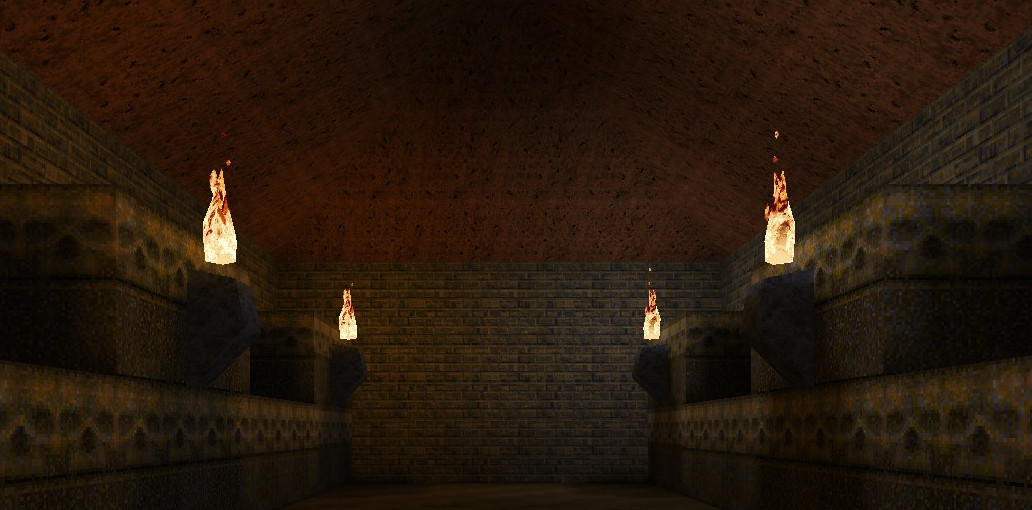
\includegraphics[width=\textwidth]{kepek/quake_torches2.jpg}
 \label{fig:quakeTorch}
\end{figure}

\subsection{Quake II (id tech 2) engine 1997}
% slow-mo explosion video: https://www.youtube.com/watch?v=L66vRF5VOVM
% md2 format: http://tfc.duke.free.fr/coding/md2-specs-en.html
A Quake motor utódjaként született meg a Quake 2 avagy az id tech 2 motor, melyen elsőként az 1997-ben megjelent Quake II játék alapult. Ez a motor már a szoftveres megjelenítés mellett az OpenGL segítségével a megjelenítés hardveres gyorsítását is támogatta. Utóbbinak köszönhetően színezett fény effektusok használata, illetve bilineáris textúra szűrés (4 pont közötti interpoláció) is lehetővé vált. Fénytérképeket itt is használtak, ám ezek már dinamikusan változtathatóak voltak. \cite{wikiQuake2, fsQuake2} Tűz megjelenítés szempontjából a Quake II játékot vizsgáltam, melyben fáklya nem volt, viszont robbanás effekt igen.

A Quake motorhoz hasonlóan a robbanás folyamata itt is előre meg van határozva képkockáról képkockára. Ebben az esetben az ilyen animált modelleket .md2 kiterjesztésű fájlokban tárolták le melyek tartalmazták:
\begin{itemize} 
\item A modell geimetriai adatait (háromszögekben)
\item A képkockáról képkockára való animációt
\item A strukturált adatokat, melyek a GL\_TRIANGLE\_FAN és GL\_TRIANGLE\_STRIP primitívek rajzolásához szükségesek OpenGL-ben.
\end{itemize} 
Az MDL formátummal ellentétben a model textúrája egy külön fájlban foglal helyet. Egy MD2 modellnek egyszerre csak 1 textúrája lehet.  \cite{MD2format}

Fizikai modellről tehát valós időben itt sem beszélhetünk. A Quake-hez képest viszont sokkal finomabb az animáció, mely arra enged következtetni, hogy a frame-ek közötti állapotokat interpolálták. Így minél nagyobb a frame-rate, annál folyékonyabb a mozgás. A robbanásokhoz tartozik dinamikus fény is. Mivel a robbanások bekövetkezése nem egy időben zajlik, egyszerre több külön modellt is meg kell jeleníteni különböző állapotokban, viszont a maximális robbanások száma egy időben 32-re van korlátozva (cl\_tent.c). A robbanás modelljén kezdetben nem lehet átlátni, de amint kibontakozik a lángcsóva, áttetszővé válik a modell és beszürkül, ami a robbanás füstjét kívánja ábrázolni. Ütközésvizsgálat nincs a lángcsóvákra, viszont a játékost visszalöki a robbanás, ha az a közelében történik. 


% 1998 Unreal engine 1
% 1999 id tech 3 engine 
% 2002 Unreal engine 2
% 2004 id tech 4 engine 
% 2004 CryEngine 1 https://github.com/AFCStudio/CRYENGINE-1
% 2007 Unreal engine 3
% 2012 Unreal engine 4 
% 2017 CRYENGINE 5.4.0 https://github.com/CRYTEK/CRYENGINE


% Not open source:
% 2012 Gamebryo 4.0  https://en.wikipedia.org/wiki/Gamebryo
% RenderWare https://en.wikipedia.org/wiki/RenderWare
% Fork_Particle https://en.wikipedia.org/wiki/Fork_Particle
% Source https://en.wikipedia.org/wiki/Source_(game_engine)
% Creation Engine https://en.wikipedia.org/wiki/Creation_Engine
% Crystal Tools https://en.wikipedia.org/wiki/Crystal_Tools
% Enigma Engine https://en.wikipedia.org/wiki/Enigma_Engine
% Frostbite https://en.wikipedia.org/wiki/Frostbite_(game_engine)
% GoldSrc https://en.wikipedia.org/wiki/GoldSrc
% IW engine https://en.wikipedia.org/wiki/IW_engine
% Jade https://en.wikipedia.org/wiki/Jade_(game_engine)
% RenderWare https://en.wikipedia.org/wiki/RenderWare
% Riot engine https://en.wikipedia.org/wiki/Riot_Engine
% RAGE https://en.wikipedia.org/wiki/Rockstar_Advanced_Game_Engine
% Vision https://en.wikipedia.org/wiki/Vision_(game_engine)#Games_using_Vision_Engine
% 2011 id tech 5 
% 2016 id tech 666

